\documentclass{article}

  % packages
    % basic stuff for rendering math
    \usepackage[letterpaper, top=1in, bottom=1in, left=1in, right=1in]{geometry}
    \usepackage[utf8]{inputenc}
    \usepackage[english]{babel}
    \usepackage{amsmath} 
    \usepackage{amssymb}
    \usepackage{natbib}

    % extra math symbols and utilities
    \usepackage{mathtools}        % for extra stuff like \coloneqq
    \usepackage{mathrsfs}         % for extra stuff like \mathsrc{}
    \usepackage{centernot}        % for the centernot arrow 
    \usepackage{bm}               % for better boldsymbol/mathbf 
    \usepackage{bbm}              % for indicator functions
    \usepackage{enumitem}         % better control over enumerate, itemize
    \usepackage{hyperref}         % for hypertext linking
    \usepackage{xr-hyper}
    \usepackage{fancyvrb}         % for better verbatim environments
    \usepackage{newverbs}         % for texttt{}
    \usepackage{xcolor}           % for colored text 
    \usepackage{listings}         % to include code
    \usepackage{lstautogobble}    % helper package for code
    \usepackage{parcolumns}       % for side by side columns for two column code
    \usepackage{algorithm}
    \usepackage{algpseudocode}

    % page layout
    \usepackage{fancyhdr}         % for headers and footers 
    \usepackage{uniquecounter} 
    \usepackage{lastpage}         % to include last page number in footer 
    \usepackage{parskip}          % for no indentation and space between paragraphs    
    \usepackage[T1]{fontenc}      % to include \textbackslash
    \usepackage{footnote}
    \usepackage{etoolbox}

    % for custom environments
    \usepackage{tcolorbox}        % for better colored boxes in custom environments
    \tcbuselibrary{breakable}     % to allow tcolorboxes to break across pages

    % figures
    \usepackage{pgfplots}
    \pgfplotsset{compat=1.18}
    \usepackage{float}            % for [H] figure placement
    \usepackage{tikz}
    \usepackage{tikz-cd}
    \usepackage{circuitikz}
    \usetikzlibrary{positioning, shapes, arrows, fit, calc}
    \usepackage{graphicx}
    \usepackage{caption} 
    \usepackage{subcaption}
    \captionsetup{font=small}

    % for tabular stuff 
    \usepackage{dcolumn}

    \usepackage[nottoc]{tocbibind}
    \pdfsuppresswarningpagegroup=1
    \hfuzz=5.002pt                % ignore overfull hbox badness warnings below this limit

  % New and replaced operators
    \DeclareMathOperator{\Tr}{Tr}
    \DeclareMathOperator{\Sym}{Sym}
    \DeclareMathOperator{\Span}{span}
    \DeclareMathOperator{\elbo}{ELBO}
    \DeclareMathOperator{\std}{std}
    \DeclareMathOperator{\Cov}{Cov}
    \DeclareMathOperator{\Var}{Var}
    \DeclareMathOperator{\proj}{proj}
    \DeclareMathOperator{\Corr}{Corr}
    \DeclareMathOperator{\pos}{pos}
    \DeclareMathOperator*{\argmin}{\arg\!\min}
    \DeclareMathOperator*{\argmax}{\arg\!\max}
    \newcommand{\ket}[1]{\ensuremath{\left|#1\right\rangle}}
    \newcommand{\bra}[1]{\ensuremath{\left\langle#1\right|}}
    \newcommand{\braket}[2]{\langle #1 | #2 \rangle}
    \newcommand{\qed}{\hfill$\blacksquare$}     % I like QED squares to be black 

  % Custom Environments
    \newtcolorbox[auto counter, number within=section]{question}[1][]
    {
      colframe = orange!25,
      colback  = orange!10,
      coltitle = orange!20!black,  
      breakable, 
      title = \textbf{Question \thetcbcounter ~(#1)}
    }

    \newtcolorbox[auto counter, number within=section]{exercise}[1][]
    {
      colframe = teal!25,
      colback  = teal!10,
      coltitle = teal!20!black,  
      breakable, 
      title = \textbf{Exercise \thetcbcounter ~(#1)}
    }
    \newtcolorbox[auto counter, number within=section]{solution}[1][]
    {
      colframe = violet!25,
      colback  = violet!10,
      coltitle = violet!20!black,  
      breakable, 
      title = \textbf{Solution \thetcbcounter}
    }
    \newtcolorbox[auto counter, number within=section]{lemma}[1][]
    {
      colframe = red!25,
      colback  = red!10,
      coltitle = red!20!black,  
      breakable, 
      title = \textbf{Lemma \thetcbcounter ~(#1)}
    }
    \newtcolorbox[auto counter, number within=section]{theorem}[1][]
    {
      colframe = red!25,
      colback  = red!10,
      coltitle = red!20!black,  
      breakable, 
      title = \textbf{Theorem \thetcbcounter ~(#1)}
    } 
    \newtcolorbox[auto counter, number within=section]{proposition}[1][]
    {
      colframe = red!25,
      colback  = red!10,
      coltitle = red!20!black,  
      breakable, 
      title = \textbf{Proposition \thetcbcounter ~(#1)}
    } 
    \newtcolorbox[auto counter, number within=section]{corollary}[1][]
    {
      colframe = red!25,
      colback  = red!10,
      coltitle = red!20!black,  
      breakable, 
      title = \textbf{Corollary \thetcbcounter ~(#1)}
    } 
    \newtcolorbox[auto counter, number within=section]{proof}[1][]
    {
      colframe = orange!25,
      colback  = orange!10,
      coltitle = orange!20!black,  
      breakable, 
      title = \textbf{Proof. }
    } 
    \newtcolorbox[auto counter, number within=section]{definition}[1][]
    {
      colframe = yellow!25,
      colback  = yellow!10,
      coltitle = yellow!20!black,  
      breakable, 
      title = \textbf{Definition \thetcbcounter ~(#1)}
    } 
    \newtcolorbox[auto counter, number within=section]{example}[1][]
    {
      colframe = blue!25,
      colback  = blue!10,
      coltitle = blue!20!black,  
      breakable, 
      title = \textbf{Example \thetcbcounter ~(#1)}
    } 
    \newtcolorbox[auto counter, number within=section]{code}[1][]
    {
      colframe = green!25,
      colback  = green!10,
      coltitle = green!20!black,  
      breakable, 
      title = \textbf{Code \thetcbcounter ~(#1)}
    } 
    \newtcolorbox[auto counter, number within=section]{algo}[1][]
    {
      colframe = green!25,
      colback  = green!10,
      coltitle = green!20!black,  
      breakable, 
      title = \textbf{Algorithm \thetcbcounter ~(#1)}
    } 
    
    \definecolor{dkgreen}{rgb}{0,0.6,0}
    \definecolor{gray}{rgb}{0.5,0.5,0.5}
    \definecolor{mauve}{rgb}{0.58,0,0.82}
    \definecolor{darkblue}{rgb}{0,0,139}
    \definecolor{lightgray}{gray}{0.93}
    \renewcommand{\algorithmiccomment}[1]{\hfill$\triangleright$\textcolor{blue}{#1}}

    % default options for listings (for code)
    \lstset{
      autogobble,
      frame=ltbr,
      language=Python,                           % the language of the code
      aboveskip=3mm,
      belowskip=3mm,
      showstringspaces=false,
      columns=fullflexible,
      keepspaces=true,
      basicstyle={\small\ttfamily},
      numbers=left,
      firstnumber=1,                        % start line number at 1
      numberstyle=\tiny\color{gray},
      keywordstyle=\color{blue},
      commentstyle=\color{dkgreen},
      stringstyle=\color{mauve},
      backgroundcolor=\color{lightgray}, 
      breaklines=true,                      % break lines
      breakatwhitespace=true,
      tabsize=3, 
      xleftmargin=2em, 
      framexleftmargin=1.5em, 
      stepnumber=1
    }

  % Page style
    \pagestyle{fancy}
    \fancyhead[L]{Machine Learning}
    \fancyhead[C]{Muchang Bahng}
    \fancyhead[R]{Spring 2024} 
    \fancyfoot[C]{\thepage / \pageref{LastPage}}
    \renewcommand{\footrulewidth}{0.4pt}          % the footer line should be 0.4pt wide
    \renewcommand{\thispagestyle}[1]{}  % needed to include headers in title page

\begin{document}

\title{Learning Theory}
\author{Muchang Bahng}
\date{Spring 2025}

\maketitle
\tableofcontents
\pagebreak

  Unlike unsupervised learning, which comes in many different shapes and forms (anomaly detection, feature extraction, density estimation, dimensionality reduction, etc.), supervised learning comes in a much cleaner format. In supervised learning, we consider an input space $\mathcal{X}$ and an output space $\mathcal{Y}$. We assume that there exists some unknown measure $\mathbb{P}$ over $\mathcal{X} \times \mathcal{Y}$, making this some probability space. We then assume that some data $\mathcal{D} = \{(x^{(i)}, y^{(i)})\}$ is generated sampled \textit{independently and identically (iid)} from $\mathbb{P}$. Now this assumption is quite strong and is almost always not the case, as different data can be correlated, but we will relax this assumption later. Let's formally construct this from the bottom up. 

  \begin{enumerate}
    \item We start off with a general probability space $(\Omega, \mathcal{F}, \mathbb{P})$. This is our model of the world and everything that we are interested in. 

    \item A measurable function $X: \Omega \rightarrow \mathcal{X}$ extracts a set of features, which we call the \textbf{covariates} and induces a probability measure on $\mathcal{X}$, say $\mathbb{P}_X$. 

    \item Another measurable function $Y: \Omega \rightarrow \mathcal{Y}$ extracts another set of features called the \textbf{labels} and induces another probability measure on $\mathcal{Y}$, the \textbf{label set}, say $\mathbb{P}_Y$. 

    \item At this point the function $X \times Y$ is all we are interested in, and we throw away $\Omega$ since we only care about the distribution over $\mathcal{X} \times \mathcal{Y}$. 

    \item We model the generation of data from $\Omega$ by sampling $N$ samples from $\mathbb{P}_{X \times Y}$, which we assume to be iid (this assumption will be relaxed later). This gives us the \textbf{dataset} 
      \[\mathcal{D} = \{(\mathbf{x}^{(i)}, \mathbf{y}^{(i)}) \}_{i=1}^N\]
  \end{enumerate}

  Now our goal is to construct a function $f: \mathcal{X} \rightarrow \mathcal{Y}$ that predicts $Y$ from $X$, but we want to define some measure of how good our function is. We can use a loss function $L$ to talk about this. 

  \begin{definition}[Risk]
    The \textbf{risk}, or \textbf{expected risk}, of function $f$ is defined as 
    \begin{equation}
      R(f) = \mathbb{E}_{X \times Y} [ L(Y, f(X))] = \int_{\mathcal{X} \times \mathcal{Y}} L(y, f(x)) \,d\mathbb{P}(x, y)
    \end{equation}
  \end{definition}

  Clearly, we don't know what this risk is since we don't know the true measure $\mathbb{P}$, so we try to approximate it with the \textit{empirical risk}. 

  \begin{definition}[Empirical Risk]
    The \textbf{empirical risk} of function $f$ is defined as 
    \begin{equation}
      \hat{R}_n(f) = \frac{1}{n} \sum_{i=1}^n L(y^{(i)}, f(x^{(i)}))
    \end{equation}
  \end{definition}

  \begin{definition}[Generlize]
    A function $f$ is said to \textbf{generalize} if 
    \begin{equation}
      \lim_{n \rightarrow +\infty} \hat{R}_n (f) = R(f)
    \end{equation}
  \end{definition}

  This gives us a way of computing with the actual data. Now two questions arise from this. First, how do we even choose the loss function $L$? Second, how do we know that the empirical risk is a good approximation of the true risk? The first question can be quite convoluted, but we introduce it with decision theory. The second has a simple answer with concentration of measure.  

\section{Decision Theory}

  How can we choose our loss functions? There are two ways of doing this, either through model assumptions or with domain knowledge. When talking about model assumptions, we assume that the residual distribution is of certain form, and the maximum likelihood formulation leads to a certain loss function. For example, assuming that the residuals are normally distributed leads to the squared loss or Laplacian residuals leads to the absolute value loss. These are just modeling assumptions, and if there are no specific assumptions, we are lost. The other way is through domain expertise which allows us to construct our own loss functions. Fortunately, there is a deeper theory behind the choice of loss functions, known as decision theory, which allows us to define loss functions from the get go rather than assume distributions taking particular forms.\footnote{Credits to Edric for telling me this.}

  \begin{definition}[Misclassification Loss]
    The \textbf{misclassification loss} is defined as 
    \begin{equation}
      L(y, \hat{y}) = \begin{cases} 0 & \text{if } y = \hat{y} \\ 1 & \text{if } y \neq \hat{y} \end{cases}
    \end{equation}
  \end{definition}

  \begin{example}[Misclassification Risk]
    Substituting the misclassification loss function into the risk gives the \textbf{misclassification risk}. 
    \begin{equation}
      R(f) = \mathbb{E} [\mathbbm{1}_{\{Y \neq f(X)\}}] = \mathbb{P}(Y \neq f(X)) 
    \end{equation}
    and therefore our empirical risk is 
    \begin{equation}
      \hat{R} (f) = \frac{1}{n} \sum_{i=1}^n \mathbbm{1}_{\{y^{(i)} \neq f(x^{(i)})\}}
    \end{equation}
    which is just the number of misclassifications over the total number of samples. 
  \end{example}

  However, depending on the context, the loss for misclassification one one label can be quite different from that of another label. Consider the medical example where you're trying to detect cancer. Falsely detecting a non-cancer patient as having cancer is not as bad as falsely detecting a cancer patient as not having cancer. 

  \begin{definition}[Weighted Misclassification Loss]
    The \textbf{loss matrix} $K$ defines the loss that we incur when predicting the $i$th class on a sample with true label $j$. 
    \begin{equation}
      L(y, \hat{y}) = \begin{cases} 0 & \text{ if } y = \hat{y} \\ K_{ij} & \text{ if } y = i \neq j = \hat{y} \end{cases}
    \end{equation}
  \end{definition}

  \begin{definition}[Squared Loss]
    The \textbf{squared loss} is defined as 
    \begin{equation}
      L(y, \hat{y}) = (y - \hat{y})^2
    \end{equation}
  \end{definition}

  \begin{example}[Mean Squared Risk]
    Substituting the squared loss function into the risk gives the \textbf{mean squared risk}. 
    \begin{equation}
      R(f) = \mathbb{E}[(Y - f(X))^2]
    \end{equation}
    and therefore our empirical risk is 
    \begin{equation}
      \hat{R} (f) = \frac{1}{n} \sum_{i=1}^n (y^{(i)} - f(x^{(i)})^2
    \end{equation}
  \end{example}

  \begin{definition}[Absolute Loss]
    The \textbf{absolute loss} is defined as 
    \begin{equation}
      L(y, \hat{y}) = |y - \hat{y}|
    \end{equation}
  \end{definition}

\section{Function Classes}

  Now that we've defined the risk and empirical risk, the true function that we want to find is the one that minimizes the empirical risk. 
  \begin{equation}
    f^\ast = \argmin_{f \in \mathcal{F}} \hat{R} (f)
  \end{equation}
  However, this depends on the function space $\mathcal{F}$ that we are minimizing over. If we chose $f$ to be the space of all functions, then we just interpolate (fit perfectly over) the data\footnote{unless there were two different values of $Y$ for the same $X$}, which is not good since we're \textbf{overfitting}. This is a problem especially in nonparametric supervised learning, and there are generally two ways to deal with this. The first is to use \textit{localization}, which deals with local smoothing methods. The second is with \textbf{regularization}. The third is to restrict our class of functions to a smaller set. Perhaps we assume that nature is somewhat smooth and so naturally we want to work with smooth functions. There are two ways that we define smoothness, through Holder spaces that focus on local smoothness and Sobolev spaces that focus on global smoothness. 

  \begin{definition}[$L^p$ Space]
    The $L^p (\mu)$ space is the normed vector space of all functions from $f: \mathcal{X} \rightarrow \mathbb{R}$ such that 
    \begin{equation}
      ||f||_p = \left( \int |f(x)|^p \,d\mu \right)^{1/p} < \infty
    \end{equation}
  \end{definition}

  \begin{theorem}[Countable Basis]
    You can construct a countable orthonormal basis in $L^2 (\mu)$ space. 
  \end{theorem}

  There are a lot of well known orthonormal bases. For example, the Fourier basis, Legendre polynomials, Hermite polynomials, or wavelets. Therefore, every function can be expressed as a linear combination of this basis, and you can calculate coefficients by taking the inner product with the basis functions. 
  \begin{equation}
    f(x) = \sum_{i=1}^\infty \alpha_i \phi_i (x) \text{ and } \alpha_i = \langle f, \phi_i \rangle
  \end{equation}

  Now we can define Holder spaces. Holder spaces are used whenever we want to talk about local smoothness. For example, when we want to talk about local smoothing methods for regression and classification, talking about this smoothing is not quite possible if we don't have certain assumptions on the function. To make theory easier, we assume that the function has basic smoothness properties and this property is Holder smoothness. But note that these are ultimately assumptions. 


  \begin{definition}[Holder Space]
    For some $\beta \in \mathbb{N}$ and $L \in \mathbb{R}^+$, the $H(\beta, L)$ \textbf{Holder space} is the set of all functions $f: \mathcal{X} \subset \mathbb{R} \rightarrow \mathbb{R}$ such that 
    \begin{equation}
      |f^{(\beta - 1)}(y) - f^{(\beta - 1)}(x)| \leq L ||y - x||
    \end{equation}
    for all $x, y$. If we want $\mathcal{X}$ to be $d$-dimensional, then we want to bound the higher order total derivatives, and so $H(\beta, L)$ becomes all functions $f: \mathcal{X} \subset \mathbb{R}^d \rightarrow \mathbb{R}$ such that for all $\mathbf{s} = (s_1, \ldots, s_d)$ with $|\mathbf{s}| = \beta - 1$,
    \begin{equation}
      |D^{\mathbf{s}} f(x) - D^{\mathbf{s}} f(x)| \leq L ||y - x||
    \end{equation}
    for all $x, y \in \mathcal{X}$, where 
    \begin{equation}
      D^{\mathbf{s}} = \frac{\partial^{|\mathbf{s}|}}{\partial x_1^{s_1} \ldots \partial x_d^{s_d}} 
    \end{equation}
    The higher $\beta$ is, the more smoothness we're demanding. 
  \end{definition}

  If $\beta = 1$, then this reduces to the set of all Lipschitz functions. It is most common to assume that $\beta = 2$, which means that the derivative is Lipschitz. This is not rigorously true, but by dividing both sides by $||y - x||$ and taking the limit to $0$, we can say that it implies that there exists some finite second derivative bounded by $L$. 

  \begin{definition}[Sobolev Space]
    The \textbf{Sobelov space} $W_{m, p}$ is the space of all functions $f \in L_p (\mu)$ such that 
    \begin{equation}
      ||D^m f||_p \in L^p (\mu)
    \end{equation}
    This is slightly stronger than the usual definition of Sobolev spaces since we requiring the derivative rather than the weak derivative. So $m$ tells us how many derivatives we want well behaved and $p$ tells us under which norm are the derivatives well behaved. 
  \end{definition}

  Now there is a related definition of a Sobelov ellipsoid that we'll be working with. 

  \begin{definition}[Sobelov Ellipsoid]
    Let $\theta = (\theta_1, \theta_2, \ldots)$ be a sequence of real numbers. Then the set 
    \begin{equation}
      \Theta_m = \bigg\{ \theta \mid \sum_{j=1}^\infty a_j^2 \theta_j^2 < C^2 \bigg\}
    \end{equation}
    where $a_j^2 = (\pi \cdot j)^{2m}$. Note that since $a_j$ is exploding, to stay finite the $\theta_j$ must be decaying.
  \end{definition}

  This is useful because of the following theorem. 
  
  \begin{theorem}[Conditions for Function being in Sobelov Space]
    Given a function $f \in L^2(\mu)$ expanded in some orthonormal basis $\phi_j$, then $f \in W_{m, 2}$ if and only if the coefficients $\alpha_j$ die off fast enough in the sense that it is in the Sobelov ellipsoid. 
  \end{theorem}

  Now let's talk about RKHS. Let's take the $L^2(\mu)$ space of functions $f: [0, 1] \rightarrow \mathbb{R}$ with $||f|| = \int f^2 \,d\mu < \infty$ and inner product $\langle f, g \rangle = \int f(x) g(x) \,d\mu$. It is known that if $f_n$ converges to $f$ in $L^2$, then it is not necessarily true that $f$ converges pointwise since it can diverge on a sequence of sets that converge to measure $0$. You probably don't want to work with functions that look like this, and that's what a RKHS is for. It gives you a nice class of functions that have good statistical properties but also are easy to compute with.  

  \begin{definition}[Mercer Kernels]
    A \textbf{Mercer kernel} is a function $K: \mathbb{R} \times \mathbb{R} \rightarrow \mathbb{R}$ that is symmetric and positive definite in the sense that for any collection $x_1, \ldots, x_n$ of arbitrary size $n$, 
    \begin{equation}
      \sum_i \sum_j c_i c_j K(x_i, x_j) \geq 0 
    \end{equation}
    which is equivalent to saying that the matrix formed by evaluating these kernels at the pairs of points is positive semi-definite. 
  \end{definition}

  \begin{example}[Gaussian Kernel]
    The Gaussian kernel is defined 
    \begin{equation}
      K(x, y) = \exp \bigg( - \frac{||x - y||^2}{\sigma^2} \bigg)
    \end{equation}
  \end{example} 

  Now this kernel should tell us roughly how similar two points $x$ and $y$ are. Using this kernel, we want to build a function space. For this, we need Mercer's theorem. 

  \begin{theorem}[Mercer's Theorem]
    If we have a kernel $K$ that is bounded 
    \begin{equation}
      \sup_{x, y} K(x, y) < \infty
    \end{equation}
    we can define a new operator $T_K$ that maps functions to functions
    \begin{equation}
      T_K f(x) =  \int K(x, y) f(y) \,dy = \iint K(x, y) f(x) f(y) \,dx\,dy
    \end{equation}
    This operator is linear, meaning that it has an eigendecomposition and therefore there exists eigenfunctions $\phi_i$ s.t. 
    \begin{equation}
      T_K \phi_i (x) = \int K(x, y) \phi_i(y) \,dy = \lambda_i \phi_i(x)
    \end{equation}
    Then these eigenvalues are bounded and we can write the kernel as a sum of the eigenfunctions. 
    \begin{equation}
      \sum_i \lambda_i < \infty, \;\;\; K(x, y) = \sum_{i=1}^\infty \lambda_i \phi_i(x) \phi_i(y)
    \end{equation}
    These $\phi_i$'s are the implicit high-dimensional features. 
  \end{theorem}

  What do these eigenfunctions $\phi_i$ look like? Well, they tend to look like functions that tend to get wigglier and wigglier as $i$ increases, indicating that $\lambda_i$ must decrease in such a way that it still keeps the function smooth. 

  Now, we can fix the first term in the kernel and it will be function of the second term $K_x (\cdot) = K(x, \cdot)$. We do this for all $x \in \mathbb{R}$, which form the basis of our RKHS, and it consists of all functions that are linear combinations of these $K_x$'s. For example, the functions 
  \begin{equation}
    f = \sum_i \alpha_i K_{x_i} \text{ and } g = \sum_j \beta_j K_{x_j} 
  \end{equation}
  can consist of a finite number of perhaps different basis functions. Now this is clearly a vector space, and to upgrade this to a Hilbert space, we must define an inner product. This inner product (with respect to some kernel $K$) is defined as 
  \begin{equation}
    \langle f, g \rangle_K = \sum_{i, j} \alpha_i \beta_j K(x_i, x_j)
  \end{equation}

  \begin{exercise}[Inner Product of RKHS]
    Show that the inner product of the RKHS is indeed an inner product.
  \end{exercise}

  The inner product induces a norm, and so by taking the completion of all linear combinations of the kernel basis functions we get our RKHS. Now since $K_x$ is itself in the RKHS, we can take the inner product of $f$ and $K_x$, which just gives us back the evaluation of $f$ at $x$. 

  \begin{definition}[Reproducing Kernel Hilbert Space]
    Given a kernel $K$, the \textbf{reprducing kernel Hilbert space} $\mathcal{H}$ is the Hilbert space of all functions $f: \mathcal{X} \rightarrow \mathcal{Y}$ that can be expressed as a linear combination of the functions $\{K_x = K(x, \cdot)\}$. It has the inner product 
    \begin{equation}
      \langle f, g \rangle_{\mathcal{H}} = \sum_{i, j} \alpha_i \beta_j K(x_i, x_j)
    \end{equation}
    and also includes all of its limit points under this norm, making it a complete space. 
  \end{definition}

  \begin{theorem}[Reproducing Property of RKHS]
    An RKHS satisfies the \textbf{reproducing property}, which means that taking the inner product of a function $f$ and a kernel $K_x$ gives you the evaluation of $f$ at $x$. 
    \begin{equation}
      \langle f, K_x \rangle_{\mathcal{H}} = f(x)
    \end{equation}
    and therefore it also means that $\langle K_x, K_x \rangle_{\mathcal{H}} = K(x, x)$. This also means that $K_x$ is the evaluation functional in the dual space of $\mathcal{H}$ and this evaluation functional $\delta_x$ is continuous, which is not always true in functional analysis.  
  \end{theorem}
  \begin{proof}
    We can evaluate from the inner product 
    \begin{equation}
      f = \sum_i \alpha_i K_{x_i} \implies \langle f, K_x \rangle_K = \sum_i \alpha_i \langle K_{x_i}, K_x \rangle_K = \sum_i \alpha_i K(x_i, x) = f(x)
    \end{equation}
  \end{proof}

  This reproducing property tends to be very useful, especially in the corollary below. 

  \begin{corollary}[Convergence in RKHS]
    Convergence in norm implies pointwise convergence in RKHS. 
  \end{corollary}
  \begin{proof}
    Given that $f_n \rightarrow f$ in norm, we have that $||f_n - f|| \rightarrow 0$. Then for all points $x \in \mathcal{X}$, 
    \begin{equation}
      |f_n(x) - f(x)| = |\langle f_n - f, K_x \rangle_{\mathcal{H}}| \leq ||f_n - f|| \cdot ||K_x|| \rightarrow 0
    \end{equation}
  \end{proof}

  \begin{theorem}[Moore-Aronszajn] 
    Any positive definite function $K$ is a reproducing kernel for some RKHS.  
  \end{theorem} 
  \begin{proof} 
    We won't be too rigorous about this since this is not a functional analysis course. Assume that we have a positive definite kernel $K: X \times X \rightarrow \mathbb{R}$, where $X$ is some measurable set, and we will show how to make a RKHS $\mathcal{H}_k$ such that $K$ is the reproducing kernel on $\mathcal{H}$. It turns out that $\mathcal{H}_k$ is unique up to isomorphism. Since $X$ exists, let us first define the set $S = \{ k_x \mid x \in X\}$ such that $k_x (y) \coloneqq K(x, y)$. Now let us define the vector space $V$ to be the span of $S$. Therefore, each element $v \in V$ can be written as 
    \[v = \sum_i \alpha_i k_{x_i}\]
    Now we want to define an inner product on $V$. By expanding out the vectors w.r.t. the basis and the properties of bilinearity, we have 
    \[\langle k_x, k_y \rangle_{V} = \bigg\langle \sum_i \alpha_i k_{x_i} , \sum_i \beta_i k_{y_i} \bigg\rangle = \sum_{i, j} \alpha_i \beta_j K(x_i, y_j)\] 
    At this point, $V$ is not necessarily complete, but we can force it to be complete by taking the limits of all Cauchy sequences and adding them to $V$. In order to complete the construction, we need to ensure that $K$ is continuous and doesn't diverge, i.e. 
    \[\iint K^2 (x, y) \,dx\,dy < +\infty\]
    which is a property known as finite trace.\footnote{Too much to write down here at this point, but for further information look at $\href{http://users.umiacs.umd.edu/~hal/docs/daume04rkhs.pdf}{the article here}$.}
  \end{proof}

  Now at first glance, this abstract construction makes it hard to determine what kind of functions there are in a RKHS generated by some kernel. Conversely, given some RKHS, it's not always easy to know which kernel it came from. 

  \begin{example}[Fourier Basis]
    Let us take the vector space of all real functions $f$ for which its Fourier transform is supported on some finite interval $[-a, a]$. This is a RKHS with the kernel function 
    \begin{equation}
      K(x, y) = \frac{\sin(a(y - x))}{a(y - x)}
    \end{equation}
    with the inner product $\langle f, g \rangle = \int f(x) g(x) \,dx$.
  \end{example}

  \begin{example}[Some Sobelov Spaces are RKHS]
    Let us take the Sobelov space $W_{1, 2}$ of all functions $f: [0, 1] \rightarrow \mathbb{R}$ satisfying 
    \begin{equation}
      \int (f^\prime (x))^2 \,dx < \infty
    \end{equation} 
    This is a RKHS with the kernel function 
    \begin{equation}
      K(x, y) = \begin{cases} 1 + xy + \frac{xy^2}{2} - \frac{y^3}{6} & \text{ if } 0 \leq y \leq x \leq 1 \\
        1 + xy + \frac{x^2 y}{2} - \frac{x^3}{6} & \text{ if } 0 \leq x \leq y \leq 1 \end{cases}
    \end{equation}
  \end{example}

  Finally, remembering Mercer's theorem, we can decompose the Kernel into its eigenfunctions 
  \begin{equation}
    K(x, y) = \sum_{j=1}^\infty \lambda_j \phi_j(x) \phi_j(y) 
  \end{equation}
  When you talk about feature maps (e.g. in support vector machines), you're really just creating the map from $x \in \mathcal{X}$ into the infinite dimensional vector space 
  \begin{equation}
    x \mapsto \Phi(x) = \big( \sqrt{\lambda_1} \phi_1(x), \sqrt{\lambda_2} \phi_2(x), \ldots \big)
  \end{equation}
  and the inner product between two functions is actually the inner product between their feature maps. Therefore, you can either just work with $x$ in the RKHS or work with the features $\Phi$ in a higher dimensional Euclidean space. Therefore, we can either work with $f$ as a combination of kerenels or a linear combination of the eigenfunctions. The eigenfunctions are easier conceptually, but when we actually do computations, the kernel expansion is much easier. 
  \begin{equation}
    f(x) = \sum_{i} \alpha_i K(x_i, x) = \sum_j \beta_j \phi_j(x) 
  \end{equation}
  When you're expanding with the eigenfunctions, you can just compute the inner product as 
  \begin{equation}
    \langle f, g \rangle = \sum_i \frac{\alpha_i \beta_i}{\lambda_i}
  \end{equation}
  and because $f, g$ must satisfy some smoothness constraints, the $\alpha_i$ and $\beta_i$ must die off quickly, making the sum finite. But we're never going to be actually computing this way since it's much easier to compute with the kernel expansion. This means that the $\phi_i$'s, which get wigglier (think of sine and cosine eigenbases) as $i$ increases, must have decreasing coefficients. 

  When working with function classes, we tend to divide them into two broad categories. 

  \begin{definition}[Parametric Models]
    A \textbf{parametric model} is a set of functions $\mathcal{M}_{\boldsymbol{\theta}}$ that can be parameterized by a finite-dimensional vector. The elements of this model are hypotheses functions $h_{\boldsymbol{\theta}}$, with the subscript used to emphasize that its parameters are $\boldsymbol{\theta}$. We have the flexibility to choose any form of $h$ that we want, and that is ultimately a model assumption that we are making. 
  \end{definition}

  \begin{example}[Examples of Parametric Models]
    \begin{enumerate}
      \item If we assume $h: \mathbb{R}^D \rightarrow \mathbb{R}$ to be linear, then $h$ lives in the dual of $\mathbb{R}^D$, which we know to be $D$-dimensional. 
      \item If we assume $h$ to be affine, then this just adds one more dimension. 
      \item If we assume $h: \mathbb{R} \rightarrow \mathbb{R}$ to be a $k$th degree polynomial, then $g$ can be parameterized by a $k+1$ dimensional $\theta$. 
    \end{enumerate}
  \end{example}

  However, parametric models may be limited in the way that we are assuming some form about the data. For certain forms of data, where we may have domain knowledge, it is reasonable to use parametric models, but there are cases when we will have absolutely no idea what the underlying distribution is. For example, think of classifying a $3 \times N \times N$ image as a cat or a dog. There is some underlying distribution in the space $[255]^{3 N^2} \times \{\text{cat}, \text{dog}\}$, but we have absolutely no idea how to parameterize this. Should it be a linear model or something else? This is when nonparametric models come in. They are not restricted by the assumptions concerning the nature of the population from which the sample is drawn. 

  \begin{definition}[Nonparametric Models]
    \textbf{Nonparametric models} are ones that cannot be expressed in a finite set of parameters. They may be countably or uncountably infinite. 
  \end{definition}

\section{Concentration of Measure}

  Concentration of measure is a tool used to prove a lot of theorems in statistical machine learning. I have another series of notes on this, but we'll stick to the key points. 

  \begin{definition}[Hoeffding's Inequality]
    Given $X_1, \ldots, X_n$ are iid random variables with $a \leq X_i \leq b$, then for any $\epsilon > 0$, 
    \begin{equation}
      \mathbb{P} \bigg( \bigg| \frac{1}{n} \sum_{i=1}^n X_i - \mathbb{E}[X] \bigg| \geq \epsilon \bigg) \leq 2 \exp \bigg( - \frac{2 n \epsilon^2}{(b - a)^2} \bigg)
    \end{equation}
  \end{definition}

  Therefore, if we apply it to some binary classifier $f: \mathcal{X} \rightarrow \{0, 1\}$, then we can say that the probability that the empirical risk deviates from the true risk is exponentially small. 
  \begin{equation}
    \mathbb{P} (|\hat{R} (f) - R(f)| \geq \epsilon) \leq 2e^{- 2 n \epsilon^2}
  \end{equation}
  But when we do empirical risk minimization (ERM), we not given a classifier, but we must \textit{choose} it. So given our space of classifiers $f$, we can plot the true risk and the noisy empirical risk. The equation above states that at any given point the probability of it deviating by more than $\epsilon$ is exponentially small. But we want something stronger: we want to bound the probability of the supremum of the difference over the whole class $\mathcal{F}$. 

  \begin{equation}
    \mathbb{P} \big( \sup_{f \in \mathcal{F}} | \hat{R} (f) - R(f) | \geq \epsilon \big)
  \end{equation}

  \begin{figure}[H]
    \centering 
    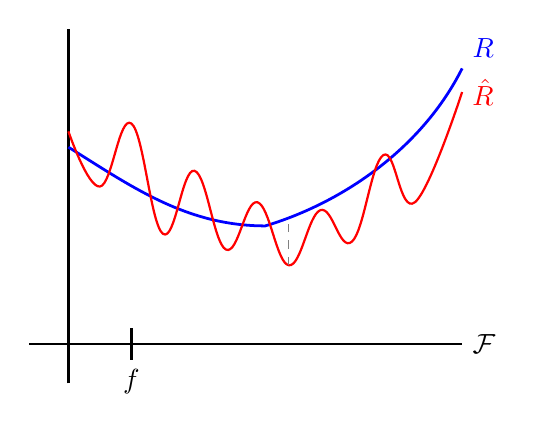
\begin{tikzpicture}
      \draw[black, line width=1pt] (-0.5,0) -- (5,0) node[right] {$\mathcal{F}$};
      \draw[black, line width=1pt] (0,-0.5) -- (0,4);

      \draw[black, line width=0.8pt] (0.8,-0.2) -- (0.8,0.2);
      \node[below] at (0.8,-0.2) {$f$};
      
      \draw[blue, line width=1pt] 
        (0,2.5) .. controls (0.8,2) and (1.5,1.5) .. 
        (2.5,1.5) .. controls (3.5,1.8) and (4.5,2.5) .. 
        (5,3.5) node[above right] {$R$};
        
      \draw[red, line width=0.8pt]
        plot[smooth, tension=0.7] coordinates {
          (0,2.7) (0.4,2.0) (0.8,2.8) (1.2,1.4) (1.6,2.2)
          (2.0,1.2) (2.4,1.8) (2.8,1.0) (3.2,1.7) (3.6,1.3)
          (4.0,2.4) (4.4,1.8) (5,3.2)
        } node[right] {$\hat{R}$};

      \draw[gray, dashed] (2.8,1.0) -- (2.8,1.6);
    \end{tikzpicture}
    \caption{True risk of functions over $\mathcal{F}$ and its noisy empirical risk. We want to bound the maximum deviation of these two over the whole class.} 
    \label{fig:true_vs_empirical_risk}
  \end{figure}

  This bound will depend on how \textit{complex} the function class $\mathcal{F}$ is, and to measure this complexity, we introduce some definitions. 

  \begin{definition}[Rademacher Complexity]
    Given \textbf{Rademacher random variables} $\sigma_1, \ldots, \sigma_n$ with $\mathbb{P}(\sigma_i = 1) = \mathbb{P}(\sigma_i = -1) = \frac{1}{2}$, the \textbf{Rademacher complexity} of a function class $\mathcal{F}$ is defined 
    \begin{equation}
      \mathrm{Rad}_n (\mathcal{F}) = \mathbb{E} \bigg[ \sup_{f \in \mathcal{F}} \bigg| \frac{1}{n} \sum_{i=1}^n \sigma_i f(Z_i) \bigg| \bigg]
    \end{equation}
    where the expectation is across the random $\sigma_i$'s and the $Z_i$'s, which are independent. 
  \end{definition}

  To get some intuition of what this is, let's consider a function class of a single function $f$. Then, the sup disappears and the term inside the absolute value sign becomes a $0$-mean random variable. Now if we have a very complex function class $\mathcal{F}$ with a lot of ``wiggly'' functions, then this value should be large. In this case, imagine a game where you pick generate some random variables $\sigma_i$ and the $Z_i$. Then, I pick a function that maximizes this value. How can I do that? If I can find a function $f$ that matches the sign of the $\sigma_i$'s ($+1$ or $-1$) at each of the values of $Z_i$, then this would be maximized. Therefore, if I have a sufficiently complex class, then I can pick a function that tracks your $\sigma_i$'s. Another way of looking at it is given noise variables $\sigma$ and $Z$, we're looking at the correlation between $\sigma$ and $f(Z)$. If we can maximize this correlation, then this is a complex class. 

  Now this is the most natural way of defining the complexity of the class, and in some cases it can be explicitly computed. However, in most cases it cannot be, but it can be bounded be something that is computable, like the VC dimension. 

  \begin{lemma}[Bigger Class, Bigger Complexity]
    If $\mathcal{F} \subset \mathcal{G}$, then $\mathrm{Rad}_n (\mathcal{F}) \leq \mathrm{Rad}_n (\mathcal{G})$.
  \end{lemma}

  \begin{lemma}[Convex Hull]
    If $\mathcal{F}$ is a convex set, then $\mathrm{Rad}_n (\mathcal{F}) = \mathrm{Rad}_n (\mathrm{conv}(\mathcal{F}))$, where $\mathrm{conv}(\mathcal{F})$ is the convex hull of $\mathcal{F}$.
  \end{lemma}

  This lemma is quite useful since if we have a certain finite set of functions, then their convex hull can encompass quite a bit, and we can also easily compute that convex hull's Rademacher complexity. Since the extremes haven't changed, the complexity doesn't change, and this might suggest that the Rademacher complexity is a good measure. 

  \begin{lemma}[Change of Complexity with Lipschitz Functions]
    Consider a $L$-Lipschitz function $g$  with $g(0) = 0$ and consider the class $\mathcal{F}$, then we can bound the class of functions $g \circ \mathcal{F} = \{ g \circ f \mid f \in \mathcal{F} \}$. 
    \begin{equation}
      \mathrm{Rad}_n (g \circ \mathcal{F}) \leq 2 L \mathrm{Rad}_n (\mathcal{F})
    \end{equation}
    This constant multiplicative bound is also useful. 
  \end{lemma}

  \begin{definition}[Projection of Function Class onto Points]
    Given a binary function class $\mathcal{F}$ with functions $f: \mathcal{X} \rightarrow \{0, 1\}$, let us denote the projection of $\mathcal{F}$ onto a set of points $z_1, \ldots, z_n \in \mathcal{X}$ to be 
    \begin{equation}
      \mathcal{F}_z = \mathcal{F}_{z_1, \ldots, z_n} = \{ (f(z_1), \ldots, f(z_n)) \mid f \in \mathcal{F} \}
    \end{equation}
    This projection determines the set of all possible binary labels that can be perfectly classified by some function $f$. 
  \end{definition}

  \begin{definition}[Shattering Number]
    The \textbf{shattering number} of $\mathcal{F}$ is defined 
    \begin{equation}
      s_n (\mathcal{F}) = s(\mathcal{F}, n) = \sup_{z_1, \ldots, z_n} |\mathcal{F}_{z_1, \ldots, z_n}|
    \end{equation}
    The highest number that this can be is $2^n$, since this is the number of possible binary vectors of length $n$. Given a set of $n$ points $z_1, \ldots, z_n$, we say that the function class $\mathcal{F}$ \textbf{shatters} this set if $\mathcal{F}_{z_1, \ldots, z_n} = |2^n|$. That is, for every one of the $2^n$ labels on the points, there exists a function that can perfectly classify them. 
  \end{definition}

  \begin{example}[Binary Functions]
    Consider the function class $\mathcal{F}$ of all binary functions of the form 
    \begin{equation}
      f(x) = \begin{cases} 1 & \text{ if } x > t \\
        0 & \text{ if } x \leq t \end{cases} 
    \end{equation}
    Then, the projection of $\mathcal{F}$ onto some $n = 3$ points is the set 
    \begin{equation}
      \{ (0, 0, 0), (0, 0, 1), (0, 1, 1), (1, 1, 1) \}
    \end{equation}
    and this is true no matter how I pick the $z_1, z_2, z_3$, and so the Shattering number is $s_n (\mathcal{F}) = 4$. 
  \end{example}

  \begin{definition}[VC Dimension]
    We know that the shattering number is bounded above by $2^n$. For $n = 1$, it is reasonable that it achieves this bound, but as $n$ grows, the Shattering number may die off. The \textbf{VC dimension} is the largest $n$ number of points that can be shattered by the function class without misclassification. 
    \begin{equation}
      n^{\mathrm{VC}} \coloneqq \sup_n \{ s_n (\mathcal{F}) = 2^n \}
    \end{equation}

    \begin{figure}[H]
      \centering 
      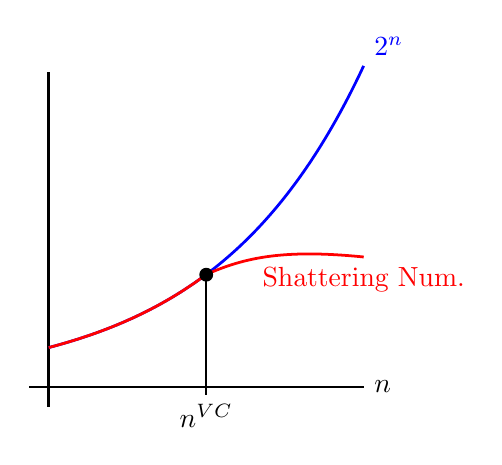
\begin{tikzpicture}[scale=0.5]
        % Draw axes
        \draw[black, line width=1pt] (-0.5,0) -- (8,0) node[right] {$n$};
        \draw[black, line width=1pt] (0,-0.5) -- (0,8);
        
        % Draw 1.1^x curve (blue)
        \draw[blue, line width=1pt] 
          plot[domain=0:8, smooth, samples=100] 
          (\x, {1.3^\x}) node[above right] {$2^n$};
          
        % Draw Shattering Number curve (red) - matches 1.1^x until VC Dim
        \draw[red, line width=1pt]
          plot[domain=0:4, smooth, samples=50] (\x, {1.3^\x})
          .. controls (5,3.3) and (6,3.5) ..
          (8,3.3) node[below] {Shattering Num.};
          
        % Mark VC Dimension / Shattering Number
        \draw[black, line width=0.8pt] (4,-0.2) -- (4,2.85);
        \node[below] at (4,-0.2) {$n^{VC}$};
        
        % Mark intersection point
        \fill[black] (4,2.85) circle (5pt);
      \end{tikzpicture}
      \caption{The Shattering number of $\mathcal{F}$ will grow exponentially until it reaches the VC dimension, at which point it will grow polynomially. The point at which it ``dies off'' is the VC dimension.} 
      \label{fig:sawyer_lemma}
    \end{figure}
  \end{definition}

  It turns out that there are very interesting properties about the VC dimension. One such fact is Sawyer's lemma, which states that if the VC dimension is finite, then the rate of growth of the shattering number suddenly changes from exponential $2^n$ to polynomial $n^{\mathrm{VC}}$, and this is what makes a lot of machine learning work. 

  \begin{definition}[Subgaussian Random Variables]
    A random variable $X$ is \textbf{subgasussian} if 
    \begin{equation}
      \mathbb{E}[e^{\lambda X}] \leq e^{\frac{\lambda^2 \sigma^2}{2}}
    \end{equation}
    Gaussians and bounded random variables are subgaussian.
  \end{definition}

  \begin{lemma}[Bound on Subgaussian Random Variables]
    Given a set of iid subgaussian random variables $X_1, \ldots, X_n$ 
    \begin{equation}
      \mathbb{E}\big[ \max_{1 \leq i \leq d} X_i \big] \leq \sigma \sqrt{2 \log d}
    \end{equation}
  \end{lemma}

  \begin{theorem}[Bound of Rademacher Complexity with Shattering Number]
    The Rademacher complexity of a binary function class $\mathcal{F}$ is bounded by 
    \begin{equation}
      \mathrm{Rad}_n (\mathcal{F}) \leq \sqrt{\frac{2 \log s_n (\mathcal{F})}{n}}
    \end{equation}
  \end{theorem}
  \begin{proof}
    Given the projection $\mathcal{F}_{z_1, \ldots, z_n}$, we can use the law of iterated expectations on the Rademacher complexity. 
    \begin{align}
      \mathrm{Rad}_n (\mathcal{F}) & = \mathbb{E} \bigg[ \sup_{f \in \mathcal{F}} \bigg| \frac{1}{n} \sum_{i=1}^n \sigma_i f(Z_i) \bigg| \bigg] \\
                                   & = \mathbb{E}_{Z} \bigg[ \mathbb{E}_{\sigma} \bigg[ \sup_{f \in \mathcal{F}} \bigg| \frac{1}{n} \sum_{i=1}^n \sigma_i f(Z_i) \bigg| \; \mid \; Z_1, \ldots Z_n \bigg] \bigg] 
    \end{align}
    Note that in the inner expectation, since $f(Z_i)$ is now fixed, then are bounding a linear combination of a bunch of $\sigma_i$'s, which are subgaussian. Using the bound above, we can reduce it to 
    \begin{equation}
      \mathbb{E}_{Z} \bigg[ \sqrt{\frac{2 \log |F_{z_1, \ldots, z_n}|}{n}}\bigg] \leq \sqrt{\frac{2 \log s_n (\mathcal{F})}{n}} \leq \sqrt{\frac{2 d \log n}{n}} 
    \end{equation}
  \end{proof}

  However, this is not the best possible bound, and in cases such as K means clustering in high dimensions, this VC bound is terrible. Now we move onto the big VC theorem which now bounds the supremum of the difference between the empirical risk and the true risk. To prove this, we need a few tricks, the first being the symmetrization trick using ghost samples. 

  \begin{lemma}[Symmetrization Lemma]
    Given a set of random variables $Z_1, \ldots, Z_n$ and a function class $\mathcal{F}$, we can define ghost samples $Z_1^\prime, \ldots, Z_n^\prime$ that are iid copies of $Z_1, \ldots, Z_n$. Then, we can bound the Rademacher complexity of the function class $\mathcal{F}$ by 
    \begin{equation}
      \mathbb{P} \bigg( \sup_{f \in \mathcal{F}} | \hat{R} (f) - R(f) | \geq \epsilon \bigg) \leq 2 \mathbb{P} \bigg( \sup_{f \in \mathcal{F}} | \hat{R} (f) - \hat{R}^\prime (f) | \geq \epsilon / 2 \bigg)
    \end{equation}
    where $\hat{R}, \hat{R}^\prime$ is the empirical risk over the original and ghost samples, respectively. 
  \end{lemma}
  \begin{proof}
    Assume that we have a function $f$ that achieves this minimum. By the triangle inequality, 
    \begin{equation}
      | \hat{R} (f) - R(f)| > t \text{ and } | \hat{R}^\prime (f) - R(f)| < \frac{t}{2} \implies | \hat{R} (f) - \hat{R}^\prime (f) | > \frac{t}{2}
    \end{equation}
    We write this again as an indicator function. 
    \begin{equation}
      \mathbbm{1} (| \hat{R} (f) - R(f)| > t, | \hat{R}^\prime (f) - R(f)| < \frac{t}{2}) \implies \mathbbm{1} (| \hat{R} (f) - \hat{R}^\prime (f) | > \frac{t}{2})
    \end{equation}
    and since the samples and the ghost samples are independent, we can take the probability over the ghost samples to get 
    \begin{equation}
      \mathbbm{1} (| \hat{R} (f) - R(f)| > t) \, \mathbb{P}_{Z^\prime} (| \hat{R}^\prime (f) - R(f)| < \frac{t}{2}) \implies \mathbb{P}_{Z^\prime} (| \hat{R} (f) - \hat{R}^\prime (f) | > \frac{t}{2})
    \end{equation}
    and the rest of the proof can be found online. 
  \end{proof}

  The reason we want this is that it removes the $R(f)$, which is some unknown true mean that can be hard to deal with since it takes infinite values. It's easier to work with two empirical risks than deal with the true risk. 

  \begin{theorem}[VC Theorem/Inequality]
    Given a binary function class $\mathcal{F}$, we have
    \begin{equation}
      \mathbb{P} \bigg( \sup_{f \in \mathcal{F}} | \hat{R} (f) - R(f) | \geq \epsilon \bigg) \leq 2 S(\mathcal{F}, n) e^{-n \epsilon^2 / 8} \approx n^d e^{-n \epsilon^2 / 8}
    \end{equation}
    You can see that the exponential term is from Hoeffding but there is an extra cost of taking the supremum over the whole function class, which is the shattering number.
  \end{theorem}
  \begin{proof}
    Given $Z_1, \ldots, Z_n \sim \mathbb{P}$, we take a new set of random variables $Z_1^\prime, \ldots, Z_n^\prime$ that are iid copies of $Z_1, \ldots, Z_n$, called \textit{ghost samples}. 
  \end{proof}

  Therefore, for some classes of sets with finite VC dimension, the shattering term will grow polynomially in $n$ but the exponential term decays faster, which is what makes this work. That's why as $n$ grows, we can get a good bound on the supremum of this difference. 

  \begin{theorem}
    With probability $\geq 1 - \delta$, we have 
    \begin{equation}
      \sup_{f \in \mathcal{F}} | \hat{R} (f) - R(f) | \leq 2 \mathrm{Rad}_n (\mathcal{F}) + \sqrt{\frac{\log (2 / \delta)}{2 n}}
    \end{equation}
  \end{theorem}

\section{Bias Variance Noise Decomposition} 

  Let's do some further analysis on this. When you take a supremum over a function class, it decomposes into 3 terms. 
  \begin{enumerate}
    \item One of which quantifies how big the function class is (more variance). 
    \item One of which quantifies the distance between the truth and the function class (bias).  
    \item One is the noise term, which is the irreducible error. 
  \end{enumerate}

  \begin{example}[Bias and Variance Tradeoff in Polynomial Regression]
    Let's motivate this by trying to fit a polynomial on some data. 
    \begin{figure}[H]
      \centering 
      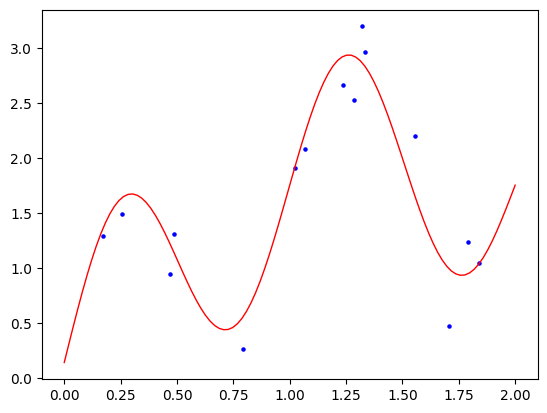
\includegraphics[scale=0.4]{img/True_data.png}
      \caption{A sample of $|\mathcal{D}| = 15$ data points are generated from the function $f(x) = \sin(2\pi x) + 2\cos (x - 1.5)$ with Gaussian noise $N(0, 0.3)$ on the interval $[0, 1]$. } 
      \label{fig:true_data}
    \end{figure}

    If we try to fit a polynomial function, how do we know which degree is best? Well the most simple thing is to just try all of them. To demonstrate this even further, I generated 10 different datasets  $\mathcal{D}$ of size $15$ taken from the same true distribution. The best fitted polynomials for each dataset is shown below. 

    \begin{figure}[H]
      \centering 
      \begin{subfigure}[b]{0.32\textwidth}
      \centering
        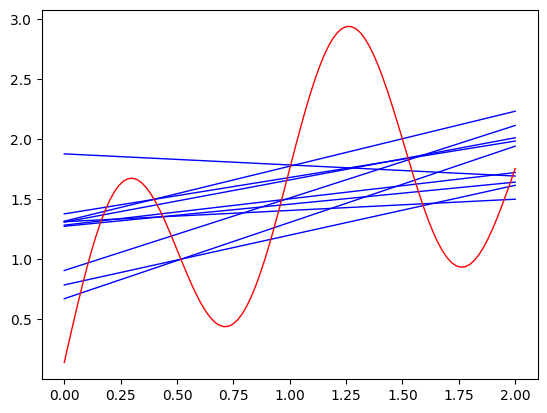
\includegraphics[width=\textwidth]{img/poly_1_fit.png}
        \caption{1st Degree}
        \label{fig:1d}
      \end{subfigure}
      \hfill 
      \begin{subfigure}[b]{0.32\textwidth}
      \centering
        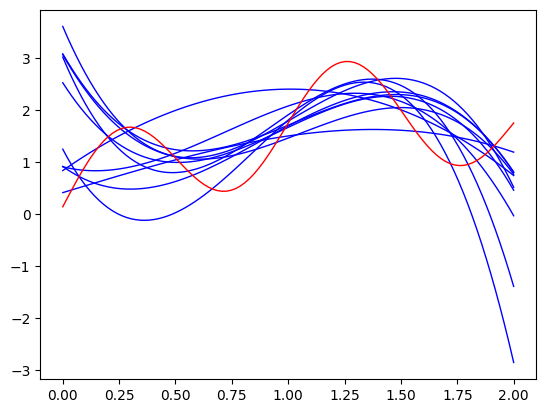
\includegraphics[width=\textwidth]{img/poly_3_fit.png}
        \caption{3rd Degree}
        \label{fig:3d}
      \end{subfigure}
      \hfill 
      \begin{subfigure}[b]{0.32\textwidth}
      \centering
        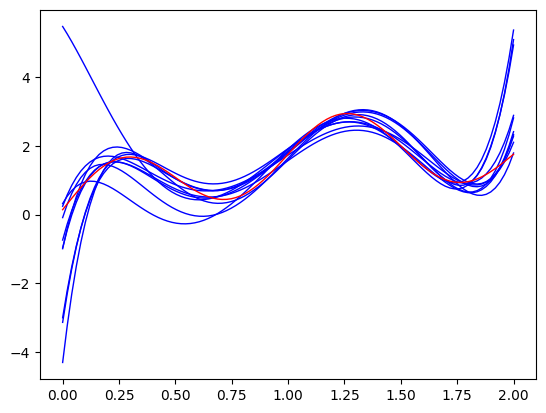
\includegraphics[width=\textwidth]{img/poly_5_fit.png}
        \caption{5th Degree}
        \label{fig:5e}
      \end{subfigure}

      \begin{subfigure}[b]{0.32\textwidth}
      \centering
        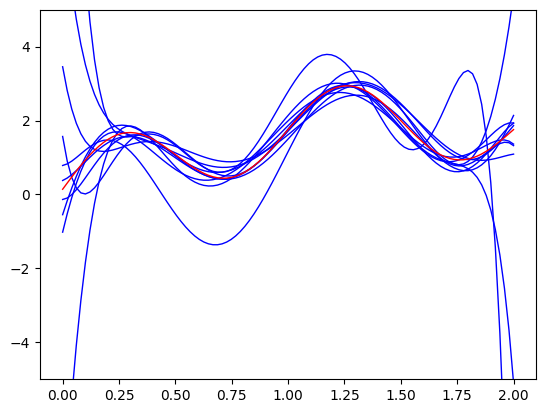
\includegraphics[width=\textwidth]{img/poly_7_fit.png}
        \caption{7th Degree}
        \label{fig:7d}
      \end{subfigure}
      \hfill 
      \begin{subfigure}[b]{0.32\textwidth}
      \centering
        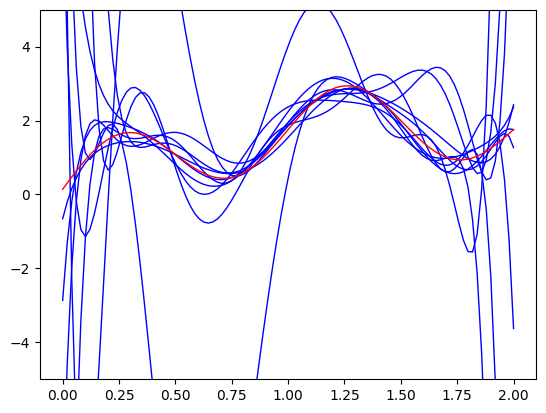
\includegraphics[width=\textwidth]{img/poly_9_fit.png}
        \caption{9th Degree}
        \label{fig:9d}
      \end{subfigure}
      \hfill 
      \begin{subfigure}[b]{0.32\textwidth}
      \centering
        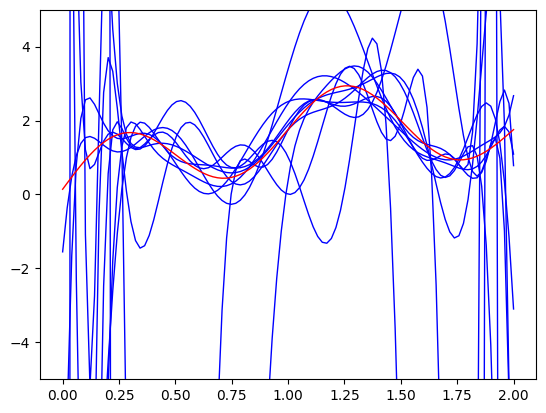
\includegraphics[width=\textwidth]{img/poly_11_fit.png}
        \caption{11th Degree}
        \label{fig:11e}
      \end{subfigure}

      \caption{Different model complexities (i.e. different polynomial degrees) lead to different fits of the data generated from the true distribution. The lower degree best fit polynomials don't have much variability in their best fits but have high bias, while the higher degree best fit polynomials have very high variability in their best fits but have low bias. The code used to generate this data is \href{code/polynomial_fitting.ipynb}{here}. }
      \label{fig:polynomial_fitting}
    \end{figure}

    We already know that the 5th degree approximation is most optimal, and the lower degree ones are \textbf{underfitting} the data, while the higher degree ones are \textbf{overfitting}. As mentioned before, we can describe the underfitting and overfitting phenomena through the bias variance decomposition. 

    \begin{enumerate}
      \item If we underfit the data, this means that our model is not robust and does not capture the patterns inherent in the data. It has a high bias since the set of function it encapsulates is not large enough to model $\mathbb{E}[Y\mid X]$. However, it has a low variance since if we were to take different samples of the dataset $\mathcal{D}$, the optimal parameters would not fluctuate. 

      \item What overfitting essentially means is that our model is too complex to the point where it starts to fit to the \textit{noise} of the data. This means that the variance is high, since different samples of the dataset $\mathcal{D}$ would cause huge fluctuations in the optimal trained parameters $\boldsymbol{\theta}$. However, the function set would be large, and thus it would be close to $\mathbb{E}[Y \mid X]$, leading to a low bias. 
    \end{enumerate}
  \end{example}
  
  \begin{example}[Polynomial Regression Continued]
    Another way to reduce the overfitting problem is if we have more training data to work with. That is, if we were to fit a 9th degree polynomial on a training set of not $N = 15$, but $N = 100$ data points, then we can see that this gives a much better fit. This makes sense because now the random variable $\mathcal{D}$, as a function of more random variables, has lower variance. Therefore, the lower variance in the dataset translates to lower variance in the optimal parameter. 

    \begin{figure}[H]
      \centering
      \begin{subfigure}[b]{0.48\textwidth}
      \centering
        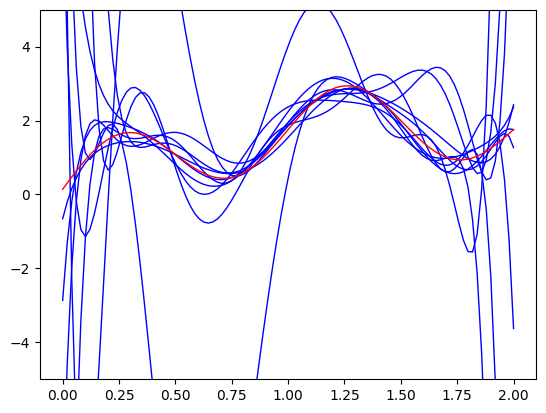
\includegraphics[width=\textwidth]{img/poly_9_fit.png}
        \caption{$M = 9, N = 15$}
        \label{fig:less_points}
      \end{subfigure}
      \hfill 
      \begin{subfigure}[b]{0.48\textwidth}
      \centering
        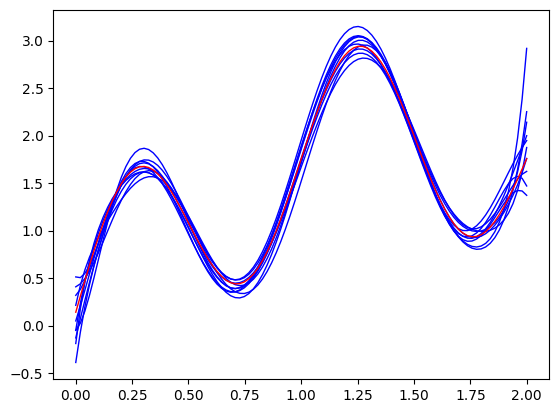
\includegraphics[width=\textwidth]{img/increased_data.png}
        \caption{$M = 9, N = 100$}
        \label{fig:more_points}
      \end{subfigure}
      \caption{Increasing the number of data points helps the overfitting problem. Now, we can afford to fit a 9th degree polynomial with reasonable accuracy.}
      \label{fig:reducing_overfitting_with_more_samples}
    \end{figure}
    
  \end{example}

\section{Minimax Theory}

\end{document}
